\documentclass[../main.tex]{subfiles} 

\begin{document}
\chapter{ASG Language}
ASG is a graphical specification language for distributed real-time systems and belongs to the family of hierarchical state languages such as \textit{STATECHARTS}, \textit{TTM} (Timed Transition Models) and \textit{MODECHARTS}. All these languages have been introduced progressively from 1987. The allow to describe the behavior of systems and have enhanced the expressiveness of state machines by introduction of time, hierarchies and parallelism. This avoids the explosion of the number of states and allows reasoning at different abstraction levels. It was intended to be readable by non computer-scientists, in order to be able to verify that what is specified is actually what the "client" wants.
\\\\
ASG, which was developed by UCLouvain, has some specific characteristics. 
\begin{itemize}
	\item It takes into account the impossibility to detect instantaneously a state change in a distributed system if it happens in a remote location (transmission delay) comment.
	\item It offers more restrictive rules on the destination state of a transition, e.g. it is not allowed to go to any other state that the initial sub-state of a state refined in sub-states if not coming from another sub-state of the same refinement. This allows to reason at a given hierarchical level without considering what happens at lower levels  comment. Consequently this promotes a top-down design, by refining states into sub-states when appropriate.
\end{itemize}

\section{Language Elements}
An ASG diagram consists of \textbf{states} and \textbf{transitions}. Crossing a transition is instantaneous: the system is thus always in a state.
\begin{figure}[H]
    \centering
    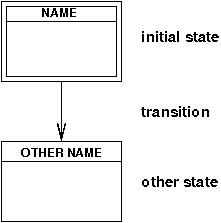
\includegraphics[width=0.25\textwidth]{asg1.jpg}
    \caption{ASG States and Transitions}
    \label{asg1}
\end{figure}

\subsection{States}
Each state has a name and some \textbf{time-related state properties:}
\begin{itemize}
	\item \textbf{MINVT}: The \textbf{minimum visit time} is the minimum time the system remains in the state.
	\item \textbf{Time-Out}: A time-out counter is started when the state is entered. When this time-out elapses, a boolean variable \texttt{state\_name.timout} becomes true if the system is still in that state. 
\end{itemize}

A state has an \textbf{action} which is executed when the state is entered. When the action is finished, the system might choose to wait in the current state.  Executing the action takes some time and can be seen as happening in parallel with the system staying in the state. An action consists of 3 steps:
\begin{enumerate}
	\item Read the necessary data
	\item Process the data
	\item Write the results atomically
\end{enumerate}
An action has one property: its \textbf{deadline}, the maximum amount of time the action is allowed to take. The deadline is a declarative temporal specification: the system should be fast enough to respect that constraint. However, since the system assumes that deadlines are always respected, it's ignored by the system and a constraint for the implementer. On the other hand, \textbf{MINVT} and \textbf{time-outs} are elements that the system's behavior has to take into account.
\\\\
Further properties of a state include a \textbf{rendez-vous label}. This is used to synchronize parallel behavior. Another propertyi is a list of \textbf{resources} to prevent parallel behavior to reach incompatible states.

\subsection{Transitions}
\begin{defn}
An \textbf{event is detected} when the system learns the following in the origin state:
\begin{center}
The system is in the origin state of the transition \textbf{and} the condition associated with the transition is true.
\end{center}
\end{defn}

\begin{figure}[H]
    \centering
    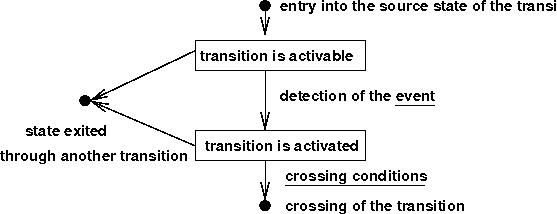
\includegraphics[width=0.5\textwidth]{asg2.jpg}
    \caption{ASG Transitions}
    \label{asg2}
\end{figure}

The condition is any boolean expression, based on environment variables or booleans indicating a \textit{rendez-vous} or \textit{time-out}. In a distributed system some time is needed in order to detect a state change of a remote variable. To avoid hidden delays the system works with local state changes and the local perception of the remote state. 
\begin{figure}[H]
    \centering
    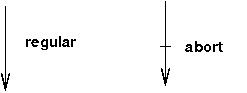
\includegraphics[width=0.3\textwidth]{asg3.jpg}
    \caption{ASG Regular and Abort Transition}
    \label{asg3}
\end{figure}
When the event is detected, the action is not necessarily finished, the time spent in the state not necessarily larger that MINVT and resources required to enter the destination state of the transition are not necessarily available. This gives cause to two families of transitions. The \textbf{crossing condition} depends on the transition family.
\begin{enumerate}
	\item  The crossing conditions of \textbf{regular transitions} (figure \ref{asg3}, left) are the following:
	\begin{itemize}
		\item The action is finished.
		\item The time spent in the state $/geq$ MINVT.
		\item All resources are available.
		\item No transition with a higher priority is active.
	\end{itemize}
	\item The crossing conditions of \textbf{abort transitions} (figure \ref{asg3}, right) is limited to the absence of a higher priority transition allowed to leave its state.
\end{enumerate}

\section{Diagram Structure}
As with similar languages, there are two ways to structure the diagrams: \textbf{parallelism} and \textbf{hierarchy}.

\subsection{Hierarchy}
\begin{figure}[H]
    \centering
    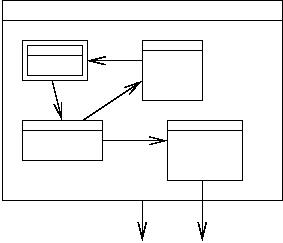
\includegraphics[width=0.4\textwidth]{asg4.jpg}
    \caption{ASG Hierarchy}
    \label{asg4}
\end{figure}
Any state may be refined in mutually exclusive sub-states. Any such sub-state is a state that may itself be refined. The system is both in the outer state as well as in the sub-state. Actions may be associated with the outer state and with each sub-state, at any level, including the initial sub-states. Action attached to the outer state and to the initial sub-state start simultaneously and are performed in parallel.
\begin{figure}[H]
    \centering
    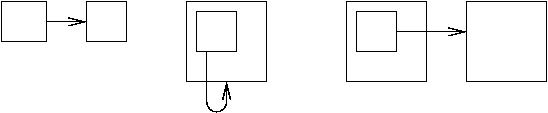
\includegraphics[width=0.6\textwidth]{asg5.jpg}
    \caption{ASG Hierarchic State Leaving}
    \label{asg5}
\end{figure}
A transition leaving a state may only end in a sister state (a state belonging to the same refinement), an ancestor state (a state enclosing the current state) or the sister of an ancestor. A state can be exited trough a transition leaving this state itself, leaving a state enclosing this state or leaving a state included in this state.
\begin{exmp}
State A could be exited trough transitions $i$, $j$ and $k$.
\begin{figure}[H]
    \centering
    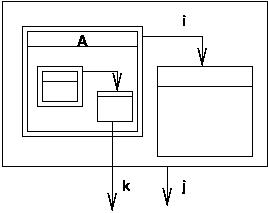
\includegraphics[width=0.4\textwidth]{asg6.jpg}
    \caption{ASG Example Leaving State}
    \label{asg6}
\end{figure}
\end{exmp}
Conditions of a transition must be satisfied for all the states that would be exited. (The system might have to wait for several actions to be completed and several MINVT to be elapsed)

\subsection{Parallelism}
In ASG, parallelism is always explicit: by entering a state that is refined into several parallel components. Exiting a state through 2 transition at a time is also not allowed in ASG.

\begin{figure}[H]
    \centering
    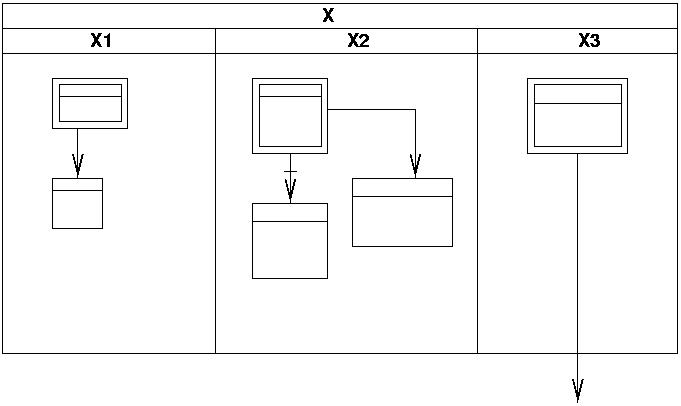
\includegraphics[width=0.6\textwidth]{asg7.jpg}
    \caption{ASG Parallelism}
    \label{asg6}
\end{figure}
When a state refined in parallel components is entered, the initial substates of all the parallel components are entered at the same time. If the refined state is exited from one of the parallel components, all the parallel components are terminated. (exiting the refined state may be through a regular or trough an abort transition)

\section{ASG Components}

\subsection{Transition Priority Rules}
One of the crossability conditions of a transition is to have the highest priority of all transitions conflicting with it. Transitions are called conflicting when they are activated and the highest state (in hierarchy) exiting is the same, or an ancestor, of the other state.

\subsection{The Rendez-Vous}
\subsection{Resources}

\section{Declarative Specificationsr}

\section{Example}



\end{document}